\chapter{Tangent Bundle}
The motivating example for tangent bundles is the case where 
$U \subset V$ is open, with $V$ a finite dimensional vector space.
A tangent vector to $p \in U$ is a vector in $V$; we write
$T_p U \simeq V$. 
\arbnote{Why write it like this? What does this mean?}
On all of $U$ the space $U \times V$ is called the 
\textbf{tangent bundle};
this is the collection of all tangent vectors on $U$. 
$TU=\bigsqcup_{p \in U} T_p U$.
$TU=U \times V$ comes with two projections:
\[ \pi : TU \to U \]
\[ S : U \to TU \]
with $\pi \circ S = \id$. The map $S$ is called a 
\textbf{vector field} on $U$.

\begin{idea}
A tangent bundle on a manifold will locally look like the above
\arbnote{What above?}
and globally describe all tangent vectors.
\end{idea}

\begin{definition}
A subspace $L \subseteq M$ of an $m$-manifold is called a 
\textbf{regular} or \textbf{embedded submanifold} of 
codimension $k$ when each point $x \in L$ is contained in a chart
$(U,\varphi)$ of $M$ such that 
\[ L \cap U = f^{-1}(0) \]
where $f$ is the composition of $\varphi$ with the projection 
$\R^m \to \R^k$ to the last $k$ coordinates 
$(x_{m-k+1}, \cdots, x_m)$. A submanifold of codimension $1$ is
called a \textbf{hypersurface}.
\end{definition}

\begin{example}
$S^n \subseteq \R^{n+1}$ is a hypersurface:
\begin{center}
\textit{(Unintelligible diagram)} 
$\displaystyle{\overset{\varphi}{\longrightarrow}}$
\Big(\parbox{3in}{\textit{A cartesian plot with a blob marked 
``$\varphi(x)$,'' ``$\iota \cap U$,'' and ``$\int$ project onto $\R$''} }\Big)
\arbnote{I can't quite tell what this means...}
\end{center}
\end{example}

Now suppose $L \subseteq \R^m$ is a submanifold of codimension $k$ and let 
$\varphi$ be a diffeomorphism as in the definition. This basically sets up a
``rectilinear'' coordinate system on $x$ where the first $m-k$ coordinates
are in $L$ and the last $k$ coordinates describe directions ``perpendicular''
to $L$. 

Then we say $u \in \R^m$ is tangent to $L$ at $p$ where the derivative $D\varphi(p)$
takes $u$ to the linear subspace of $\R^m$ given by $x_{m-k-1} = \cdots = x_m = 0$.
\arbnote{Why the ellipsis?}
Then the tangent bundle $TL$ to $L$ is the set $y$ pairs $(p,u)$ where $p \in L$ and 
$u \in \R^m$ is tangent to $L$ at $p$. It is a subset of $T \R^m=\R^m \times \R^m$ 
and is itself a submanifold of $T \R^m$ of codimension $2k$.

\begin{figure}[h]
\centering
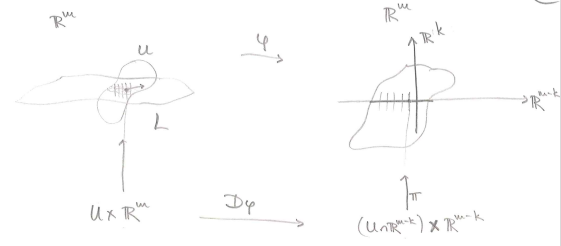
\includegraphics[width=\textwidth]{im/02-00-p28-pic}
\caption{A diagram found on page 28 of the handwritten notes.}
\end{figure}

\section{The general Construction}

\section{The Derivative}

\input{ch/sec02-03}
\input{ch/sec02-04}
